\documentclass{article}

\usepackage{full page}

\usepackage{listings}
\usepackage{color}

\definecolor{mygreen}{rgb}{0,0.6,0}
\definecolor{mygray}{rgb}{0.5,0.5,0.5}
\definecolor{mymauve}{rgb}{0.58,0,0.82}

\lstset{ %
  backgroundcolor=\color{white},   % choose the background color; you must add \usepackage{color} or \usepackage{xcolor}
  breakatwhitespace=false,         % sets if automatic breaks should only happen at whitespace
  breaklines=true,                 % sets automatic line breaking
  captionpos=b,                    % sets the caption-position to bottom
  commentstyle=\color{mygreen},    % comment style
  deletekeywords={...},            % if you want to delete keywords from the given language
  escapeinside={\%*}{*)},          % if you want to add LaTeX within your code
  extendedchars=true,              % lets you use non-ASCII characters; for 8-bits encodings only, does not work with UTF-8
  frame=none,                    % adds a frame around the code
  keepspaces=true,                 % keeps spaces in text, useful for keeping indentation of code (possibly needs columns=flexible)
  keywordstyle=\color{blue},       % keyword style
  language=Java,                 % the language of the code
  morekeywords={*,...},            % if you want to add more keywords to the set
  numbers=none,                    % where to put the line-numbers; possible values are (none, left, right)
  showspaces=false,                % show spaces everywhere adding particular underscores; it overrides 'showstringspaces'
  showstringspaces=false,          % underline spaces within strings only
  showtabs=false,                  % show tabs within strings adding particular underscores
  stringstyle=\color{mymauve},     % string literal style
  tabsize=2,                       % sets default tabsize to 2 spaces
  title=\lstname                   % show the filename of files included with \lstinputlisting; also try caption instead of title
}

\usepackage[pdftex]{graphicx}
\usepackage{float}
\usepackage{caption}
\usepackage{subcaption}
\lstset{language=Java}

\title{Chess AI}
\author{Michelle Shu}

\begin{document}
\maketitle

\section{Introduction}

Games such as chess comprise an interesting class of search problems in which an opponent introduces uncertainty into the search by producing unpredictable actions. The goal of a good game-playing agent is to produce the best possible move in a domain of limited information, and also to produce the decision efficiently within a given time limit. Here I will discuss how the minimax algorithm is used to intelligently play the game of chess. I will then address the following techniques that can be added to minimax to optimize the search within the allotted time constraint:

\begin{itemize}
\item Alpha beta pruning enables us to avoid exploring sections of the search tree that will not affect the final result.
\item Evaluation functions are heuristics which allow us to estimate the value of a chess position, even if it is not a terminal one.
\item Transposition tables allow us to store information about positions we have previously visited, so we can avoid exploring from them again on subsequent encounters.
\end{itemize}

\section{Minimax Search Algorithm}

The minimax algorithm can be applied to zero-sum multiplayer games, including chess. It is a method that an agent may use to choose actions in the game, relying on the premise that the players have opposite goals and that all players will play optimally to maximize their chance at arriving at a goal state. The minimax algorithm works toward the goal of maximizing a utility value of the game (that reflects its proximity to a winning terminal state). Additionally, it assumes that its opponent is trying to minimize the same utility value. Hence, the game tree is composed of alternating layers of max nodes and min nodes connected by edges representing game moves, where the value of a max node is the maximum of its children's values and the value of a min node is the minimum of its children's values (Fig. 1).

The minimax algorithm proceeds in the following major steps:

\begin{enumerate}
\item Generate the entire search tree up to maximum depth of search
\item Use the evaluation function (heuristic) to estimate assign utility values to all leaf nodes of the tree.
\item Move up the tree one layer at a time, determining parent nodes' utility values by taking either the min or max of children nodes, depending on the type of node.
\item When the root node is reached, return the action that leads to the child node with the highest utility value.
\end{enumerate}

The minimax player chooses the move for which its opponent can do the least damage by selecting the action that will result in the highest expected utility from the current state (represented by the root of the search tree). For instance, in Fig. 1, the minimax player will choose the move that leads to the state represented by its middle child (min node with value 9) to achieve the maximum utility value of 9.

\begin{figure}[!htb]
\centering
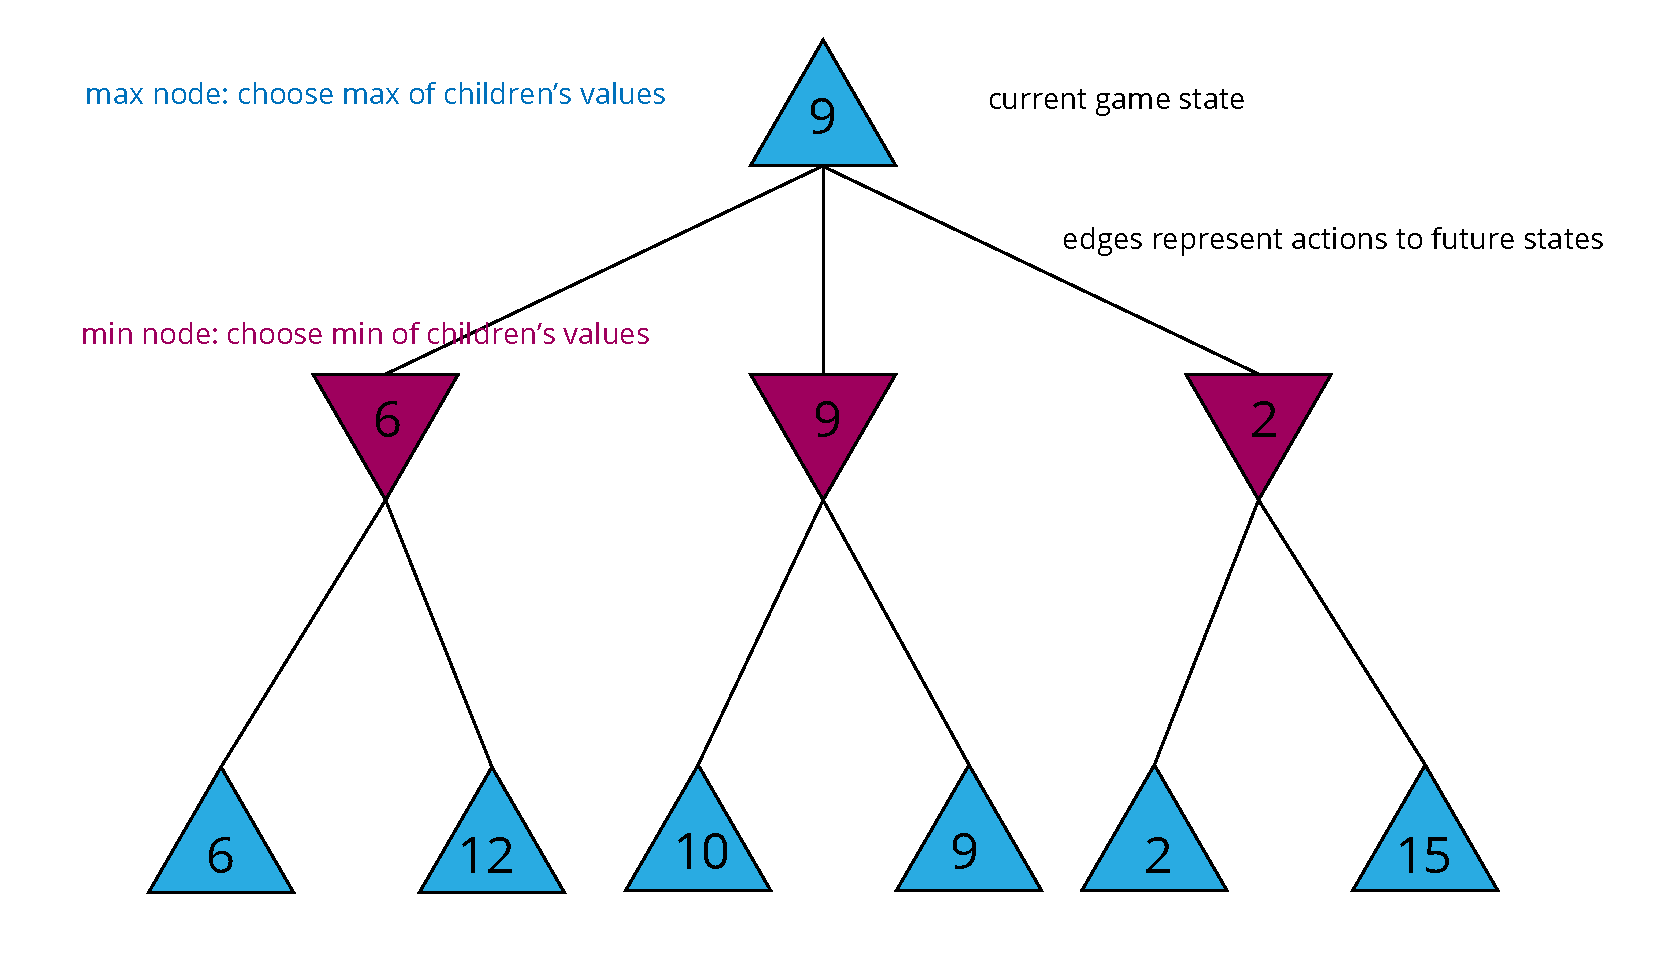
\includegraphics[scale=0.6]{minimaxtree.pdf}
\caption{{\bf Minimax Tree}}
\end{figure}

In the optimal scenario, the computer would be able to explore the minimax tree all the way down to its terminal nodes (nodes representing the end of the game). But for the game of chess, this is computationally infeasible towards the beginning of a game, due to the sheer number of possibilities that would have to be explored. Therefore, we must limit the depth of exploration to ensure that this search is tractable.

\section{Depth-Limited Minimax Implementation}

I implemented the minimax algorithm recursively. The processing of all nodes of the search tree with the exception of the root node is done with the functions \verb`maxValue` for max nodes and \verb`minValue` for min nodes in \verb`MinimaxAI.java`. Effectively, a depth-first search is done on the game tree and the max/min utility values of a node are determined as the recursion unwinds. Each node is passed a chess position to explore from, the current depth of exploration and the depth at which to cut off the search.

\vspace{5mm}

\begin{lstlisting}
private int maxValue(Position position, int depth, int cutoffDepth) {
  if (cutOffTest(position, depth, cutoffDepth)) {
    return utility(position);
  }
  int maxValue = - Integer.MAX_VALUE;
  short[] moves = position.getAllMoves();
  for (int i = 0; i < moves.length; i++) {
    short m = moves[i];
    try {
      position.doMove(m);
      maxValue = Math.max(maxValue, minValue(position, depth + 1, cutoffDepth));
      // Undo the move on original position so that we can try another
      position.undoMove();
    } catch(IllegalMoveException e) {
      System.out.println("Tried illegal move in minimax.");
    }
  }
  return maxValue;
}
\end{lstlisting}

\vspace{5mm}

\begin{lstlisting}
private int minValue(Position position, int depth, int cutoffDepth) {
  if (cutOffTest(position, depth, cutoffDepth)) {
    return utility(position);
  }
  int minValue = Integer.MAX_VALUE;
  short[] moves = position.getAllMoves();
  for (int i = 0; i < moves.length; i++) {
    short m = moves[i];
    try {
      position.doMove(m);
      minValue = Math.min(minValue, maxValue(position, depth + 1, cutoffDepth));
      // Undo the move on original position so that we can try another
      position.undoMove();
    } catch(IllegalMoveException e) {
      System.out.println("Tried illegal move in minimax.");
    }
  }
  return minValue;
}
\end{lstlisting}

\vspace{5mm}

If we reach a leaf node at a depth equal to the cutoff depth, we use the heuristic function \verb`utility` to evaluate the utility of the node. I first chose a rudimentary utility function that returns appropriate values for terminal states(high value for win, low value for loss, medium for stalemate) and a random value for everything else. An improvement to this heuristic will be discussed in the {\it Evaluation Functions} section.

\vspace{5mm}

\begin{lstlisting}
private int utility(Position position) {
  nodesExplored++;
  if (position.isTerminal()) {
    if (position.isMate()) {
      if (position.getToPlay() == this.color) {
        // I lose b/c opponent just checkmated me
        return - Integer.MAX_VALUE;
      } else {  // I win!
        return Integer.MAX_VALUE;
      }
    } else {  // no one wins
      return 0;
    }
  } else {
    return rand.nextInt(Integer.MAX_VALUE) - (Integer.MAX_VALUE / 2);
  }
}
\end{lstlisting}

\vspace{5mm}

The top-level function called from the current game state (root node) is a variation of \verb`maxValue` that, in addition to finding the highest utility child node found, tracks the move that leads to optimal path. 

\vspace{5mm}

\begin{lstlisting}
private void getMoveAtDepth(Position position, int cutoffDepth) {
  int value;
  short[] moves = position.getAllMoves();
  for (int i = 0; i < moves.length; i++) {
    short m = moves[i];
    try {
      position.doMove(m);
      value = minValue(position, 1, cutoffDepth);
      
      if (value > bestMoveValue) {
        bestMove = m;
        bestMoveValue = value;
      }
      position.undoMove();
    } catch(IllegalMoveException e) {
      System.out.println("Tried illegal move in minimax.");
    }
  }
}
\end{lstlisting}

\section{Iterative Deepening Minimax}

When asked to generate the next move, the chess AI may not know how deep it can explore before the time runs out and it must return the best move found. To explore up to the maximum depth possible in the allotted time frame, we use an iterative deepening approach, in which a search is done on each possible cutoff depth, starting with 1 and becoming progressively deeper. In the function \verb`getMove`, the iterative deepening search is implemented by placing a loop around minimax searches set at steadily increasing cutoff depths.

 \begin{lstlisting}
public short getMove(Position position) {
  // Reset bestMoveValue for this search
  bestMoveValue = - Integer.MAX_VALUE;
  
  if (position.isTerminal()) { return Move.NO_MOVE; }  // Game over
  for (int cutoffDepth = 1; cutoffDepth <= this.finalDepth; cutoffDepth++) {
    getMoveAtDepth(position, cutoffDepth);
    // At any time, if timer runs out before we explore at finalDepth, 
    // return the best value we have found in allotted time.
  }
  return bestMove;
}
\end{lstlisting}

\subsection{Results: Finding Mate in 2}

The minimax algorithm should select the moves leading up to a checkmate if it is given the opportunity to win the game within its search horizon. Because the search explores the complete set of possibilities up to its maximum depth, minimax is expected to encounter the winning position and assign it the maximum utility value, and proceed to choose moves leading up to it. This is precisely what happens in the Mate-in-2 scenario described in Figure 2, when it is explored at a depth of 3.

\begin{figure}[!htb]
\centering
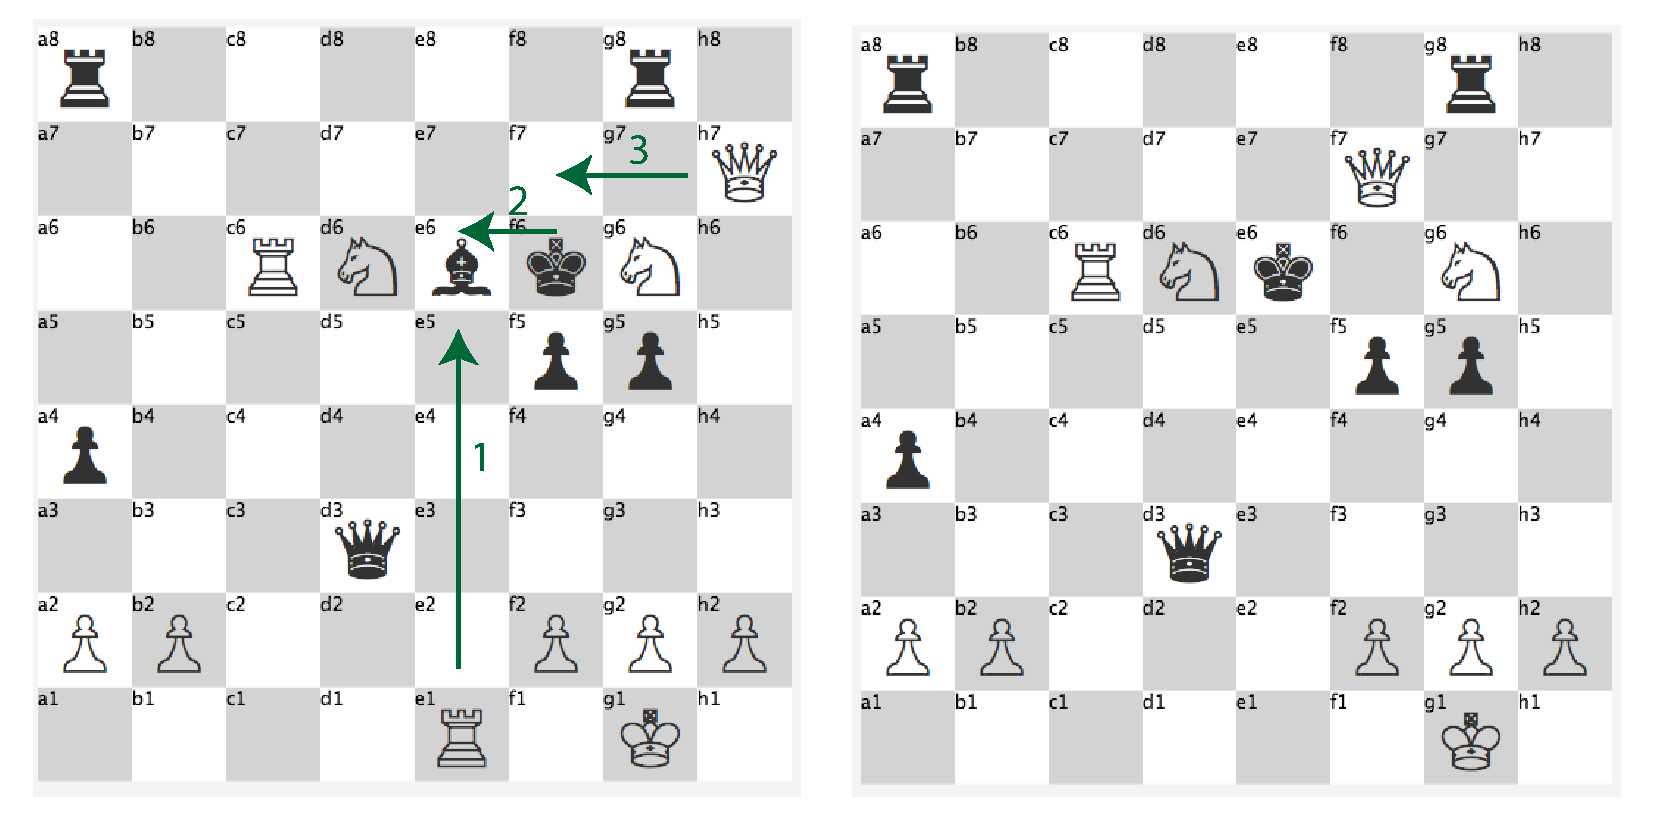
\includegraphics[scale=0.65]{mateintwo.pdf}
\caption{Mate in Two}
\end{figure}

Here is the minimax player's (white player's) evaluation of maximum utility in its first and second move as it looks ahead to depth 3. As we expect, in the first search, it finds the checkmate with value 2147483647 at 3 moves away from the current position. Then in the second search, it's next move is decidedly the one that results in a checkmate.

\vspace{20mm}

{\setlength{\parindent}{0cm}
White move 1:\\
Best move found at depth 1 has value 1072884021\\
Best move found at depth 2 has value 1072884021\\
Best move found at depth 3 has value 2147483647\\
Check!\\

\vspace{5mm}

White move 2:\\
Best move found at depth 1 has value 2147483647\\
Best move found at depth 2 has value 2147483647\\
Best move found at depth 3 has value 2147483647\\
Check!\\
Checkmate!\\}

We can roughly estimate how the speed of the search varies with different cutoff depths of search by counting the number of nodes explored in the search tree at each depth. The following analysis takes the average of the number of nodes explored in the first 5 moves of a game at various depths. (The number of actions available varies at different stages of the game, with less at the start and end of the game, so I just chose to compare the first 5 moves from start of the game here.) The numbers below demonstrate that the time required to complete a search of the game tree grows exponentially in relation to the cutoff depth.

\vspace{5mm}

{\setlength{\parindent}{0cm}
Average number of nodes explored in first 5 moves of game:\\
Depth 1: 57.8\\
Depth 2: 1,769.4\\
Depth 3: 68,628.6\\
Depth 4: 1,086,709.8\\
Depth 5: 32,812,052.4\\
Depth 6: 906,909,722.0}

\section{Evaluation Functions}

As it stands, the minimax algorithm simply generates a random utility score for non-terminal nodes. We can further improve the performance of the program by defining an evaluation function, a heuristic that reflects the relative chance of winning from the current position. A good evaluation function will allow us to make locally optimal moves that get us closer to a checkmate, even if the winning terminal state is far beyond the horizon of the search.

\subsection{Material Utility}

Material utility is a method to score the current pieces on the board irrespective of their positions, weighted by relative values. It simply sums the scores of the current player's pieces and subtracts those of the opponent's pieces. Here is my implementation of \verb`getMaterialUtility` in \verb`EvaluationFunctions.java`:

\begin{lstlisting}
public static int getMaterialUtility(Position position, int color) {
  // Count differences in number of pieces on board (black - white)
  int pawnd, knightd, bishopd, rookd, queend, kingd, stone;
  pawnd = knightd = bishopd = rookd = queend = kingd = 0;
  for (int col = 0; col < 8; col++) {
    for (int row = 0; row < 8; row++) {
      stone = position.getStone(Chess.coorToSqi(col, row));
      switch (stone) {
        case 1 : knightd++;
          break;
        case -1 : knightd--;
          break;
        case 2 : bishopd++;
          break;
        case -2 : bishopd--;
          break;
        case 3 : rookd++;
          break;
        case -3 : rookd--;
          break;
        case 4 : queend++;
          break;
        case -4 : queend--;
          break;
        case 5 : pawnd++;
          break;
        case -5 : pawnd--;
          break;
        case 6 : kingd++;
          break;
        case -6 : kingd--;
          break;
        default : break;
      }
    }
  }
  // Assign relative weights from ChessBin.com
  int utility = (975 * queend) + (500 * rookd) + (325 * bishopd) + 
      (320 * knightd) + (100 * pawnd) + (32767 * kingd);
  
  if (color == Chess.WHITE) { // white's perspective
    utility = - utility;
  }
  if (utility == 0) { // level playing field, just randomize it a little
    Random rand = new Random();
    return rand.nextInt(20) - 10;
  }
  return utility;
}
\end{lstlisting}

I observed that using the material evaluation function improved the performance of minimax. There was more strategy involved in how the minimax AI played the game, as it preferentially chose the moves that led to capturing its opponent's pieces and avoided moves that resulted in its own pieces being captured.

\section{Alpha Beta Pruning}

It is possible to choose the best possible move in the minimax search process without exploring every node of the search tree. This is the main idea behind alpha-beta pruning, which selects the same move as a full minimax search would, but prunes away branches of the tree that are irrelevant to finding the optimal move. For any node in the search tree, if a player has a better option higher up in the tree (i.e. ancestor of node will not be chosen), there is no need to explore this node because it will never be encountered in the game.

In alpha-beta pruning, we define $\alpha$ represents the maximum value we have found so far on a path for the max player and $\beta$ represents the minimum value we have found so far on a path for the min player. If a max node encounters a child with a value less than $\alpha$, it can ignore that child. Similarly, if a min node encounters a child with a value greater than $\beta$, it can ignore that child.

Here is are the revised \verb`maxValue` and \verb`minValue` functions in \verb`AlphaBetaAI.java` necessary to utilize the values of $\alpha$ and $\beta$.

\begin{lstlisting}
private int maxValue(Position position, int alpha, int beta, int depth, int cutoffDepth) {
  if (cutOffTest(position, depth, cutoffDepth)) {
    return utility(position);
  }
  int maxValue = - Integer.MAX_VALUE;
  short[] moves = position.getAllMoves();
  for (int i = 0; i < moves.length; i++) {
    short m = moves[i];
    try {
      position.doMove(m);
      maxValue = Math.max(maxValue, minValue(position, alpha, beta, depth + 1, cutoffDepth));
      position.undoMove();
      if (maxValue >= beta) {
        return maxValue;
      }
      alpha = Math.max(alpha, maxValue);
    } catch(IllegalMoveException e) {
      System.out.println("Tried illegal move in alpha beta minimax.");
    }
  }
  return maxValue;
}
\end{lstlisting}

\begin{lstlisting}
private int minValue(Position position, int alpha, int beta, int depth, int cutoffDepth) {
  if (cutOffTest(position, depth, cutoffDepth)) {
    return utility(position);
  }
  int minValue = Integer.MAX_VALUE;
  short[] moves = position.getAllMoves();
  for (int i = 0; i < moves.length; i++) {
    short m = moves[i];
    try {
      position.doMove(m);
      minValue = Math.min(minValue, maxValue(position, alpha, beta, depth + 1, cutoffDepth));
      position.undoMove();
      if (minValue <= alpha) {
        return minValue; 
      }
      beta = Math.min(beta, minValue);
    } catch(IllegalMoveException e) {
      System.out.println("Tried illegal move in alpha beta minimax.");
    }
  }
  return minValue;
}
\end{lstlisting}

While alpha-beta pruning does not improve on the result of minimax search, it allows for faster decisions to be made and thus, for exploration at deeper depths within the same time constraint. The deeper the exploration, the farther out the horizon of the search, and thus better searches can be made by using alpha-beta and continuing deeper into the search tree.

We can see the advantage of pruning by comparing the number of nodes explored in each move as an agent using minimax with alpha-beta pruning plays against an agent using minimax without alpha-beta pruning, both using iterative deepening search to a maximum depth of 6. Taking the average of the first 5 moves of the game, we find that using alpha-beta pruning clearly speeds up the efficiency of the search, as less nodes need to be explored.

\vspace{5mm}

{\setlength{\parindent}{0cm}
Average number of nodes explored in first 5 moves of game:\\
Alpha Beta nodes explored: 5,639,642.0\\
Minimax nodes explored: 861,165,179.8}

\section{Transposition table}

A transposition table is a hash table that is used to record chess positions that were previously encountered in the search, along with the depth at which they were found at and the utility value computed for them. This process of memoizing our search will greatly help in speeding up future \verb`getMove` queries. From here on out, every time we try to search from a position in the minimax tree, we first look up the position in our transposition table. If an transposition table entry exists and the utility value is accurate enough for the current query, we simply use the memoized value and don't accrue the computational costs of doing a full recursive minimax search from the node. 

We consider the stored utility value accurate enough if it was computed at a sufficient depth. For instance, if the utility value was last computed by exploring 4 layers down in the minimax tree, it can be reused by any search that would otherwise explore $\le 4$ layers. However, if the subsequent search would go $\ge 5$ layers deeper, we would continue with the standard recursive minimax search to compute a more accurate value.

I defined a packet class called \verb`TEntry` to contain the two units of information needed for a position's entry in the transposition table: the depth at which it was found and the corresponding utility value computed:

\begin{lstlisting}
public class TEntry {
	public int depth;
	public int utility;
	public TEntry(int d, int u) {
		depth = d;
		utility = u;
	}
}
\end{lstlisting}

Here are the updates done on my recursive \verb`maxValue` function 

Adding the transposition table significantly improved the time efficiency of the minimax search.

\section{References}

Chess Programming Wiki. http://chessprogramming.wikispaces.com/

Marina Sirota, Francine Anene and Eric Mayefsky. "Strategies and Tactics for Intelligent Search". \\*http://www.stanford.edu/\textasciitilde msirota/soco.

\end{document}

